\setchapterpreamble[ur][.6\textwidth]{%
\dictum[Eiji Yoshikawa, \textit{Musashi} (1935)]{
The world is always full of the sound of waves. The little fishes, abandoning themselves to the waves, dance and sing, and play, but who knows the heart of the sea, a hundred feet down? Who knows its depth?
}\vskip1em}


\chapter[\texorpdfstring{Chapter 4 \\ The stasis that wasn't: Adaptive body mass evolution is opposite to phenotypic selection in a wild rodent population}{Chapter 4 -- The stasis that wasn't: Adaptive body mass evolution is opposite to phenotypic selection in a wild rodent population}]{The stasis that wasn't: Adaptive body mass evolution is opposite to phenotypic selection in a wild rodent population}
\chaptermark{The stasis that wasn't}
\label{chap:stasis}

\textbf{Timoth\'{e}e Bonnet*}, Peter Wandeler, Glauco Camenisch and Erik Postma. In review for PloS Biology. 

\section{Abstract}
Despite being heritable and under selection, trait dynamics often do not appear to match those predicted by evolutionary theory. Indeed, conclusive evidence for contemporary adaptive evolution of quantitative traits remains rare for wild vertebrate populations, and stasis seems to be the norm. 
This so-called `stasis paradox' highlights our inability to predict evolutionary change. This is especially concerning within the context of rapid anthropogenic environmental change, and its underlying causes are therefore hotly debated.
Applying a quantitative genetic framework to individual-based long term data for a wild rodent population, we show that in this population stasis is an illusion: The population has evolved to become lighter, and this genetic change is an adaptive response to a change in snowfall patterns. Whereas both this evolutionary change and the selective pressures that drive it are not apparent on the phenotypic level, by estimating selection at the genetic level we were able to identify the relevant phenotypic selective pressure, as well as uncover the accompanying evolutionary response.
We thereby demonstrate that natural populations can show a rapid and adaptive evolutionary response to novel selective pressures, and that explicitly (quantitative) genetic models are able to provide us with an understanding of the causes and the consequences of selection that is superior to purely phenotypic estimates of selection and evolutionary change.


\section[Introduction]{Introduction}

Given the rapid anthropogenic environmental changes experienced by organisms around the world, there is an increasing need for an ability to understand and predict the evolutionary dynamics of wild populations \parencite{parmesan2006,Merila2014}. Despite good empirical examples of the adaptive evolution of traits with a simple genetic architecture \parencite{vantHof2011,Karell2011,Lamichhaney2016}, the picture is very different for quantitative traits, which are are a function of many genes of small effect \parencite{Wellenreuther2016}. Although it are these traits that are of most interest to evolutionary biologists \parencite{Roff2007, Walsh2014}, predictive models of quantitative trait evolution have largely failed when applied to data from wild populations \parencite{Merila2001}. 

Although there is an abundant literature showing that both directional selection \parencite{Kingsolver2001, Kingsolver2012} and heritable genetic variation \parencite{Mousseau1987,Postma2014} are common, these pre-requisites of Darwinian evolution rarely allow us to explain evolutionary trends retrospectively, let alone to make predictions for the future \parencite{Merila2001, Morrissey2012sts}. For example, both natural and sexual selection almost universally favour larger and heavier individuals \parencite{Blanckenhorn2000}. Furthermore, morphological traits are generally moderately heritable \parencite{Mousseau1987, Postma2014}, and averaged across the 151 estimates compiled in \parencite{Postma2014}, the heritability of body mass is  $0.33\pm0.02$. Nevertheless, while species do tend to get larger over geological timescales \parencite{Cope1887,Alroy1998,Heim2014,Baker2015}, this rate of evolution is orders of magnitude slower than what could be predicted from the strength of selection and heritability observed in contemporary populations \parencite{Merila2001, Bell2010a, Gotanda2015}.

On the whole, conclusive evidence for the contemporary adaptive evolution of quantitative traits in wild vertebrate populations is remarkably scarce and elusive \parencite{Merila2001,Morrissey2012sts}, and good examples \textemdash Trinidadian guppy life-histories \parencite{Reznick1996}, human reproductive timing \parencite{Milot2011}, timing of pink salmon migration \parencite{Kovach2012} and big-horn sheep horn size \parencite{Pigeon2016}\textemdash can be counted on one hand. Furthermore, of these studies, \parencite{Pigeon2016} reported a response to harvesting-induced, artificial rather than natural selection, and despite considerable effort to uncover any evolutionary consequences of climate change \parencite{Charmantier2014climate,Gienapp2014,Merila2014,Crozier2014}, only \parencite{Kovach2012} were able to demonstrate an adaption to climate. 

Our apparent inability to reconcile predictions of evolutionary change based on estimates of selection and genetic variation with the (lack of) of genetic change observed, i.e. the `stasis paradox' \parencite{Merila2001}, is a major concern in urgent need of a resolution. Given how commonly evolutionary predictions fail to capture observed trait dynamics, some have concluded that there are fundamental problems that prohibit the application of quantitative genetic methods to natural populations \parencite{Steiner2012,Coulson2015}. However, there are in fact three theoretically well-developed (quantitative genetic) explanations for this mismatch. 

First, although the great majority of studies base their observed rate of evolution solely on phenotypic changes, evolutionary change does not need to be apparent at the phenotypic level. Instead, it may be masked by phenotypically plastic changes, which may be several-fold larger and/or go opposite to the genetic change \parencite{Postma2007a}. For instance, while a change in the environment may generate selection favouring an increase in the frequency of alleles promoting fat accumulation, at the same time this may create a food shortage, leading to a plastic decrease of fat reserves. As a consequence, an evolutionary trend may be masked by a counteracting plastic change, also referred to as ``cryptic evolution'' \parencite{Merila2001a,Hadfield2011}. 

Second, this potentially flawed phenotypic estimate of the the \emph{observed} rate of evolution is typically compared to a \emph{prediction} derived from the univariate breeder's equation, i.e. the product of selection and heritability, where selection is quantified as the covariance between the trait of interest and relative fitness. In natural systems, selection however rarely acts on traits in isolation \parencite{Lande1983}. If these traits are genetically correlated to the focal trait, they may significantly alter the focal trait's evolutionary trajectory \parencite{Schluter1991, Morrissey2012constraints}. While the role of genetic correlations among traits within the same individual \parencite{Teplitsky2014} or between the sexes \parencite{Poissant2010} has received substantial attention, the potential role of genetic constraints resulting from genetic correlations between traits expressed in different individuals has received far less attention. In particular parent-offspring conflict, i.e. a genetic trade-off between offspring quality and fecundity \parencite{Trivers1974}, may however constrain the evolution of size \parencite{Kolliker2015}, with positive directional selection on offspring size counterbalancing selection against investment per offspring on the level of parents \parencite{Rollinson2015b}. 

Finally, even in the absence of selection on correlated traits, it is challenging to obtain an estimate of the strength of natural selection that is unbiased by the existence of a third, non-genetic variable that influences both the trait and fitness \parencite{Rausher1992}. Although the univariate breeder's equation assumes that the covariance between phenotype and fitness is solely the result of a causal relationship between the two \parencite{Morrissey2010,Morrissey2012sts}, this assumption is likely to be violated, especially in natural populations. For instance, a trait that plastically responds to food availability, such as body mass,  is likely to covary with fitness at the phenotypic level, irrespective of the causal effects of the trait on fitness: individuals that have access to more food are heavier and reproduce more \parencite{VanNoordwijk1988a,Schluter1991}. Because the fitter individuals are not genetically different in terms of body mass, this covariation has no evolutionary consequences, even if body mass is heritable \parencite{Rausher1992}. 

While these difficulties have been discussed previously, and studies regularly note that the mismatch between the observed and predicted response may be attributable to any of them, they rarely account for them in an explicit, quantitative manner. Therefore, we here apply a comprehensive analytical framework to long-term individual-based body mass data for a wild rodent population, which shows an apparent mismatch between observed rates of phenotypic change and predicted rates of genetic change. We use information on within-population relatedness and individual-level trait measurements \parencite{Henderson1950,Lynch1998} to obtain a statistically robust estimate of the direction and rate of genetic change \parencite{Postma2006,Hadfield2010b,Morrissey2012sts}. Subsequently we disentangle the role of genes and the environment in shaping the covariance between body mass and fitness, and identify the target of selection. This allows us to directly compare the observed genetic change to a range of evolutionary predictions, and to thereby resolve the stasis paradox and provide a deeper understanding of selection and evolution in this biological system. 

\section{Results and discussion}
Based on ten years of data on an alpine population of snow voles \parencite{Garcia-Navas2015,Bonnet2016} (\textit{Chionomys nivalis}, Martin 1842), we find that relatively heavy individuals both survive better ($p=0.04$) and produce more offspring per year ($p=0.003$). Assuming causality, this generates a strong phenotypic estimate of selection favouring heavier individuals (selection differential $S=0.86$ g, $p< 10^{-5}$). In line with other morphological traits \parencite{Mousseau1987,Postma2014}, variation in body mass has a significant additive genetic component ($V_A$=4.34 g$^2$, 95\%CI [2.40;7.36]), which corresponds to a heritability ($h^2$) of 0.21 (95\%CI [0.11;0.29]). Similarly, we find significant additive genetic variance in fitness ($V_A$=0.10; 95\%CI [0.06;0.19], $h^2=0.06$ 95\%CI [0.04;0.12]), measured as relative lifetime reproductive success (rLRS).

\begin{figure}[h]
\begin{center}
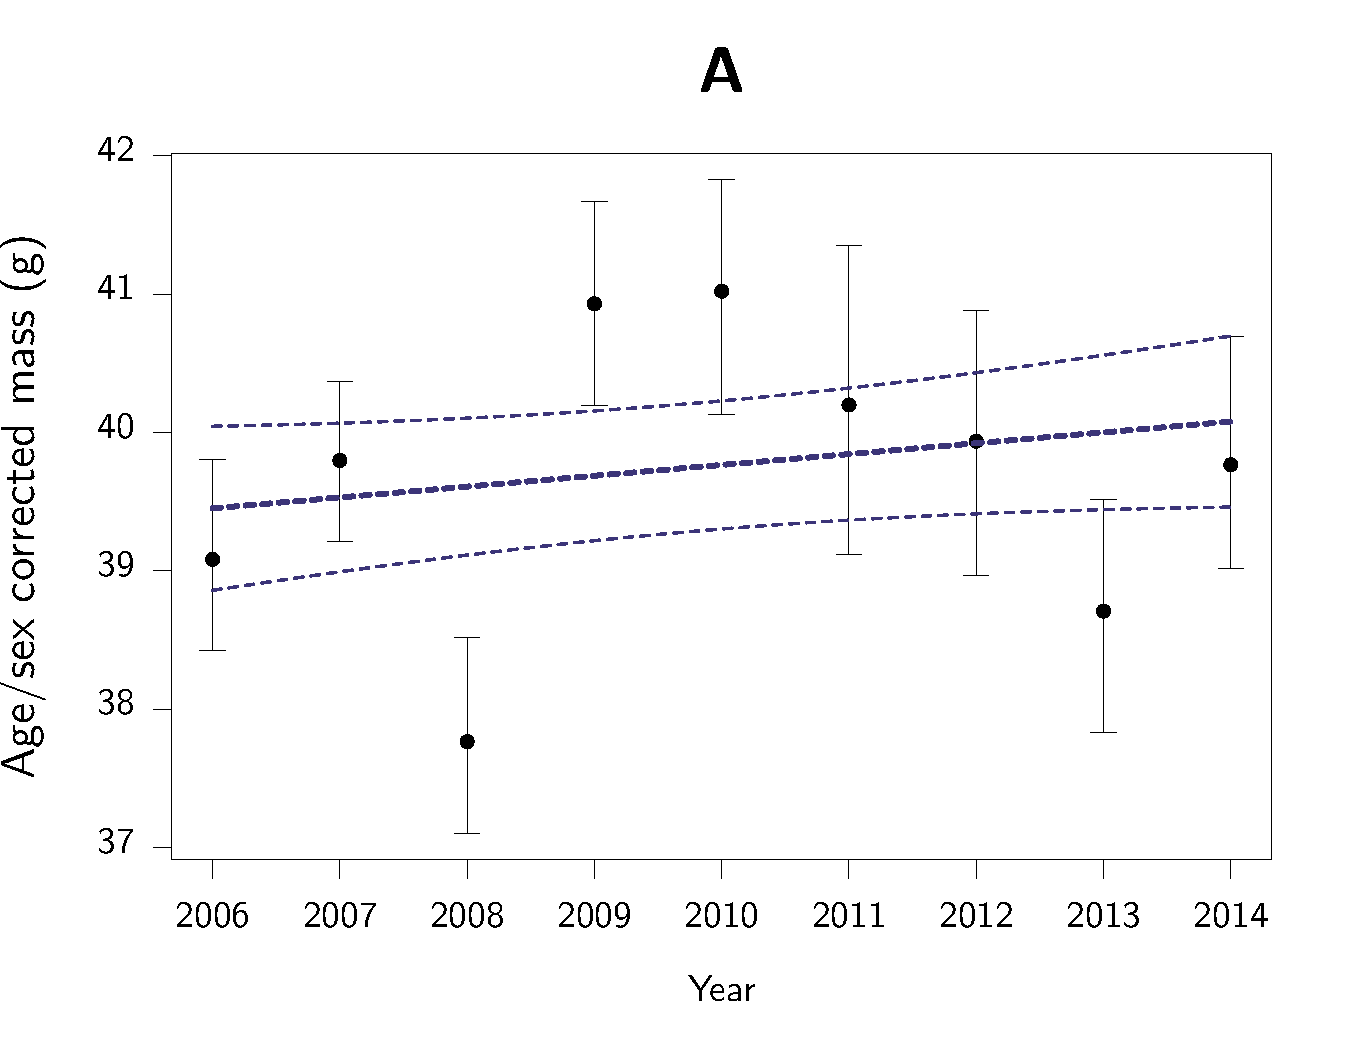
\includegraphics[width=0.49\textwidth]{FiguresStasis/PhenoTrends-1}
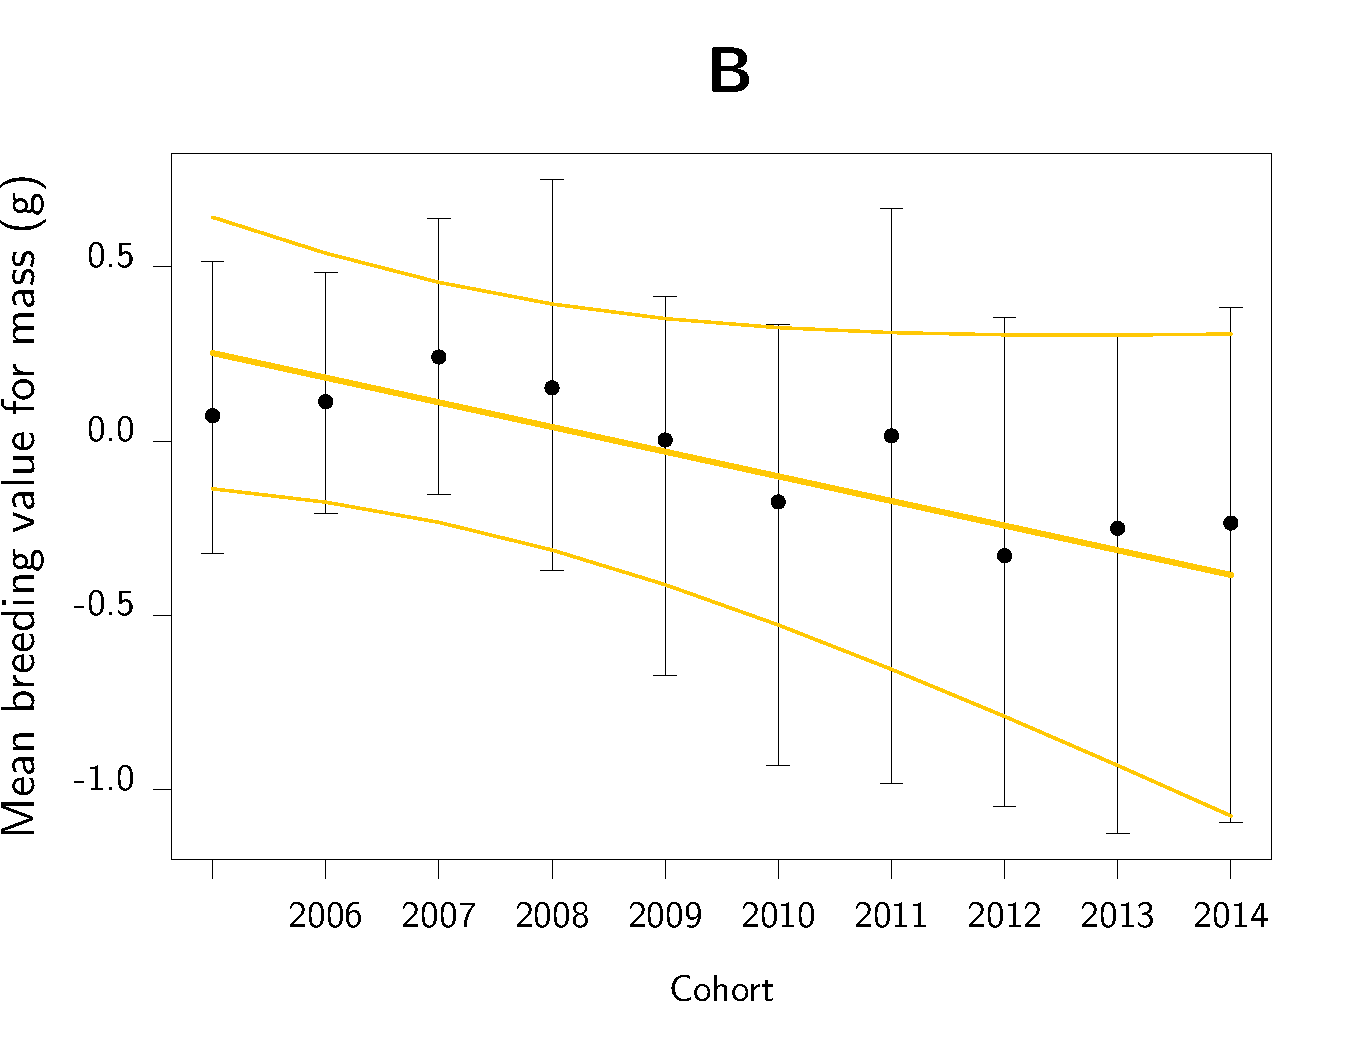
\includegraphics[width=0.49\textwidth]{FiguresStasis/BlupsTrendMass-1}
\end{center}
\caption{\footnotesize\textbf{Temporal variation in mass and estimated breeding values for mass.} (\textbf{A}): Year-specific mean mass corrected for age, sex and date of measurement, with 95\%CI. (\textbf{B}): Cohort-specific mean estimated breeding value for mass with their 95\%CI and the trend in breeding value with 95\%CI. Note the different of scale on the y-axes.}
\label{fig:trends}
\end{figure}


Given these estimates of selection ($S$) and heritability ($h^2$), the breeder's equation ($R=h^2S$) predicts an adaptive evolutionary response ($R$) in body mass \parencite{Lynch1998,Morrissey2012sts}, i.e. an increase in the mean breeding value for body mass over time, of 0.17 g/year (95\%CI [0.07;0.28]; Fig. \ref{fig:gch}A UBE).  However, after correcting for changes in demographic structure (i.e. accounting for sex and age effects, see Fig. \ref{fig:pop}), over the past nine years (approximately eight generations), the change in mean body mass is not significant and small at best (0.08 g/y; 95\%CI [-0.02;0.18]; p=0.14). This apparent mismatch between the predicted evolutionary change based on the breeder's equation and the phenotypic change observed provides yet another example of the stasis paradox \parencite{Merila2001}.

To test whether the predicted positive genetic trend, i.e. an increase in breeding values, is being masked by an opposing phenotypically plastic response \parencite{Merila2001,Hadfield2011}, we directly estimated the additive genetic covariance between mass and fitness. Based on the Robertson-Price's equation, this provides an unbiased estimate of the rate of genetic change per generation \parencite{Robertson1966,Price1970,Morrissey2012sts}. Contrary to our prediction, this estimate of genetic change in mass is strongly negative and highly significant ($p_\mathrm{MCMC}<0.001$; Fig. \ref{fig:gch}A GCPE). When normalized by a mean generation time of 1.2 years, this provides a rate of evolutionary change of -0.29 g/year (95\%CI [-0.55; -0.07]) or approximately 8,600 Darwins, which is in line with other rates of ``micro-evolution'' (e.g. between 3,700 and 45,000 Darwins in the Trinidadian guppies \parencite{Reznick1997}). Importantly, this rate of evolution is unlikely to have happened solely through genetic drift ($p_\mathrm{MCMC}<0.001$; Fig. \ref{fig:drift} and \ref{fig:driftcomp}) \parencite{Hadfield2010b}, and therefore most likely reflects a response to selection favouring genetically lighter individuals. 

\begin{figure}[ht]
{\centering
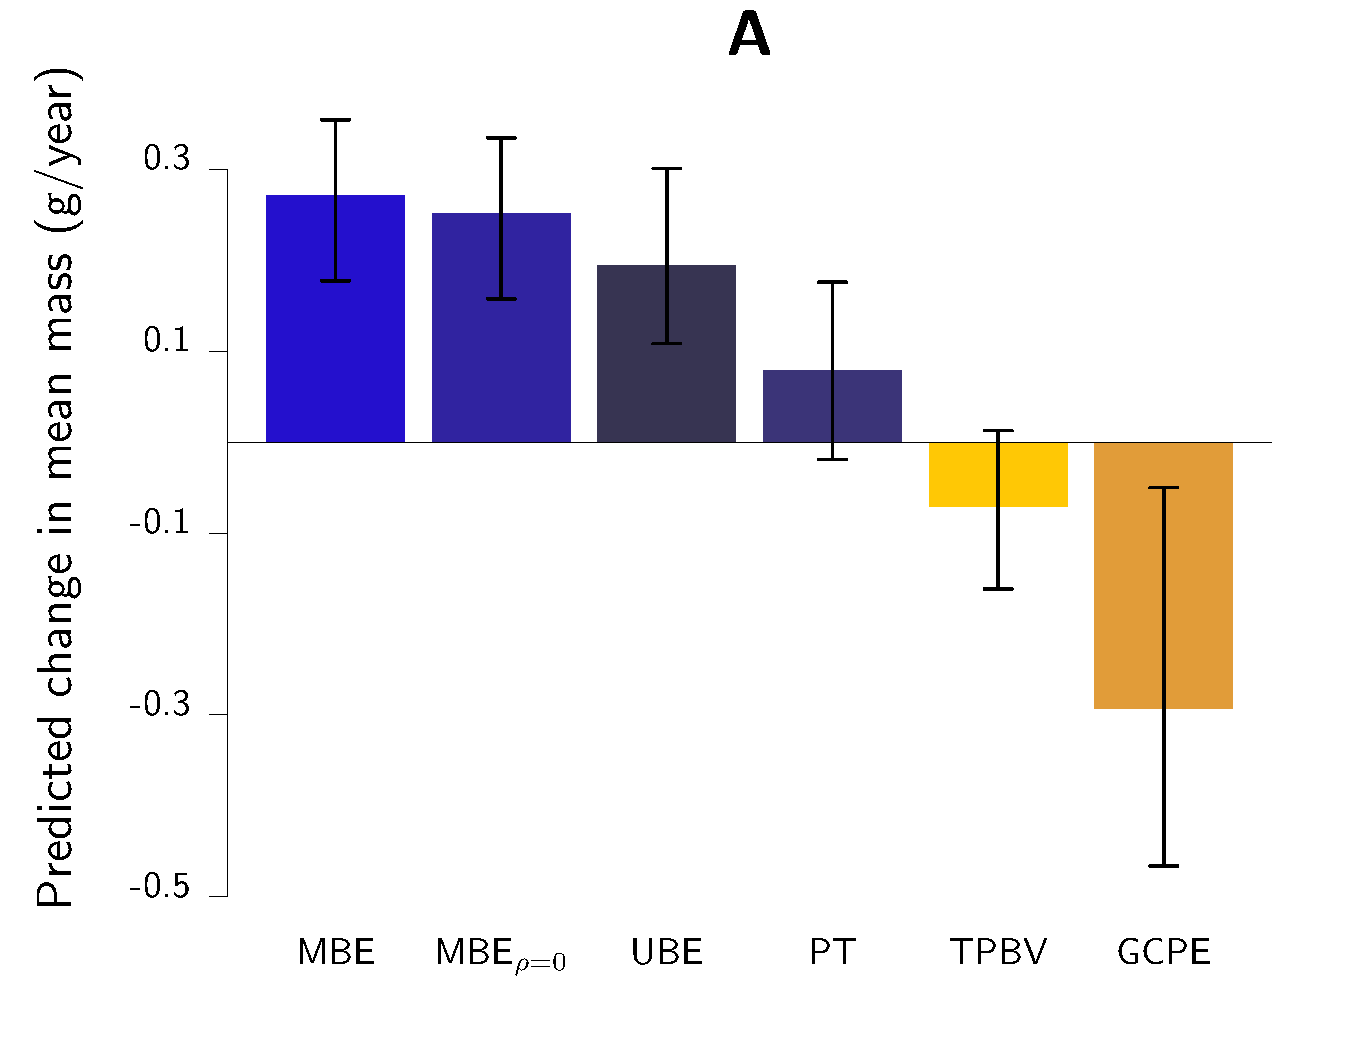
\includegraphics[width=0.49\textwidth]{FiguresStasis/AllChangeMass-1}
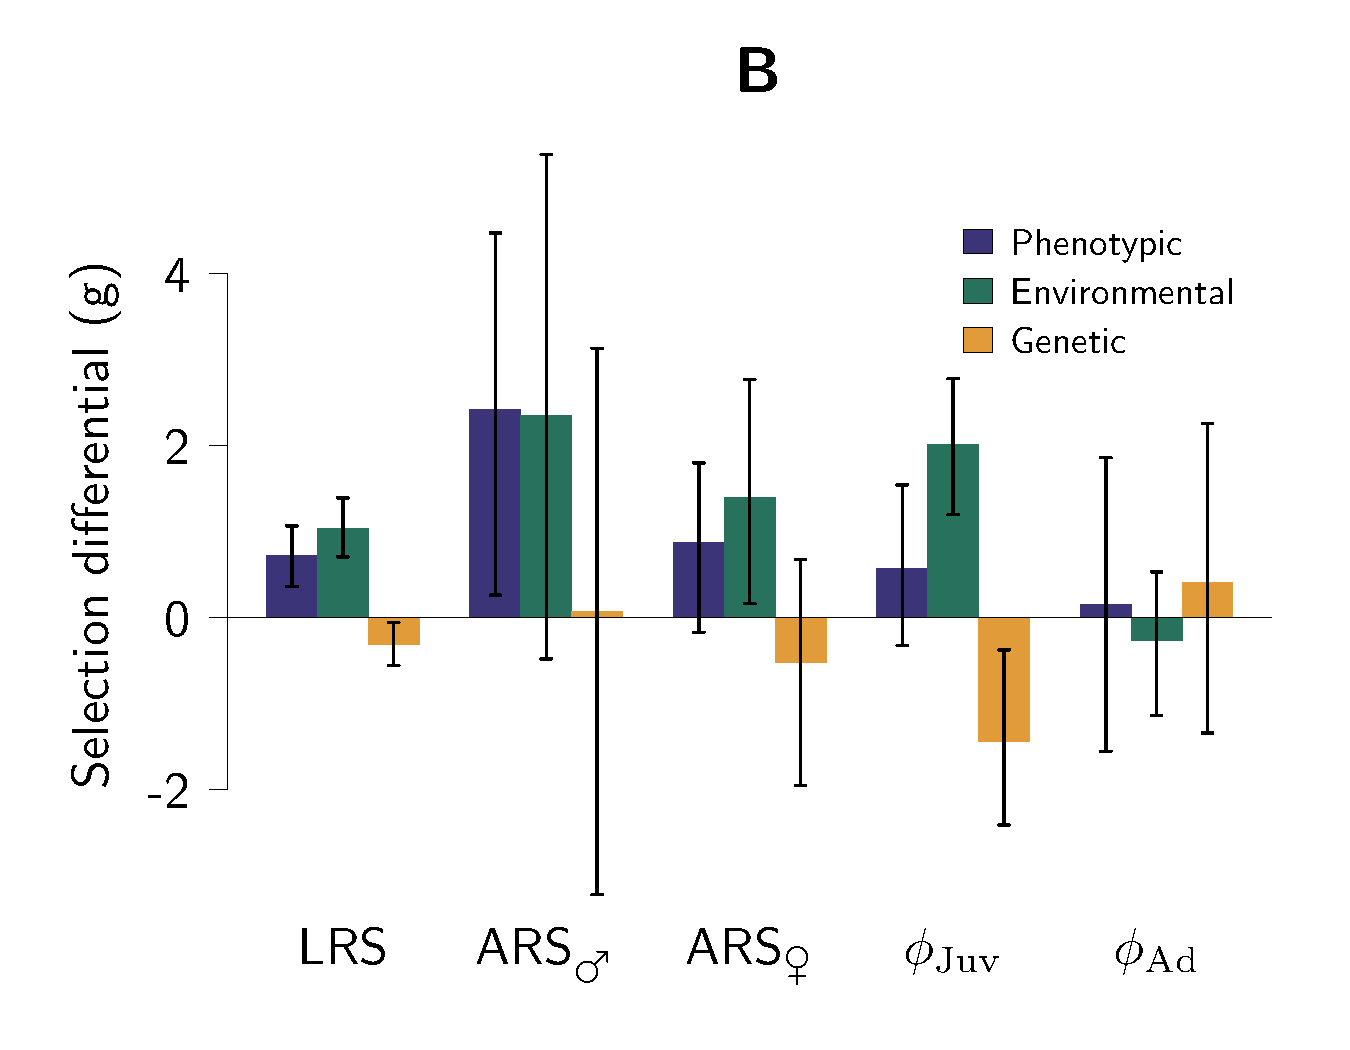
\includegraphics[width=0.49\textwidth]{FiguresStasis/SelectionS-1}
}
\caption{\footnotesize \textbf{Predicted and observed rates of evolutionary change.} (\textbf{A}): Rates of evolutionary change predicted by (from left to right) the breeder's equation in its multivariate form (MBE), the multivariate breeder's equation while constraining the genetic correlations to zero (MBE$_{\rho=0}$), and the univariate breeder's equation (UBE), followed by the phenotypic trend (PT), the trend in predicted breeding values (TPBV) and the genetic change estimated by the Price equation (GCPE). (\textbf{B}): Phenotypic, genetic and environmental selection differential for total selection (LRS), fertility selection in males (ARS$_{\male}$) and females (ARS$_{\female}$), viability selection in juveniles ($\phi_\mathrm{Juv}$) and in adults ($\phi_\mathrm{A}$). Both panels show posterior modes, with vertical lines indicating 95\%CI.}
\label{fig:gch}
\end{figure}

This result was confirmed by an independent estimate using best linear unbiased predictors (BLUPs) of breeding values for mass: Taking into account the non-independence of BLUPs and sampling variance \parencite{Postma2006,Hadfield2010b}, we find that predicted breeding values have declined over the past nine years (-0.07 g/year, $p_\mathrm{MCMC}$=0.06; Fig. \ref{fig:trends}B \& Fig. \ref{fig:gch}A TPBV), and this despite the BLUPs approach being potentially biased towards the phenotypic trend \parencite{Postma2006} (i.e. in this case toward zero). This negative trend, combined with the fact that the phenotypic mean has either remained constant or has shown a slight increase (see above), implies that the plastic component of body mass must have increased. Although the cause of this increase remains unknown, population size has declined over the study period (Fig. \ref{fig:pop}), which may have resulted in an increase in the per-capita resource availability (i.e. density dependence). Alternatively, the absolute food availability or quality may have improved. Interestingly, although these environmental changes may be coincidental, they may also be a direct result of a change in the selection regime or the evolutionary change toward smaller size \parencite{Cooke1990, Hadfield2011}.

As the phenotypic selection differential ($\sigma_{P(m,\omega)}$) is equal to the sum of the additive genetic and environmental covariances between mass and rLRS ($\sigma_{A(m,\omega)}$ and $\sigma_{E(m,\omega)}$, respectively) \parencite{Robertson1966,Price1970,Morrissey2012sts}, it follows that because $\sigma_{P(m,\omega)}$ is positive and $\sigma_{A(m,\omega)}$ is negative, the environmental covariance must be large and positive (Fig. \ref{fig:gch}B LRS). In other words, while environmental conditions that make voles heavy (for instance abundance of food or lack of parasites) also make them successful at reproducing and surviving, there is no causal \emph{positive} relationship between breeding values for mass and fitness (Fig. \ref{fig:HypA}). It is this difference in sign between $\sigma_{A(m,\omega)}$ and $\sigma_{E(m,\omega)}$ which represents an extreme violation of the breeder's equation (which assumes ${\sigma_{A(m,\omega)}}/({\sigma_{A(m,\omega)}+\sigma_{E(m,\omega)}})=h^2$). Hence, our initial prediction of evolution was wrong, demonstrating that phenotypic estimates of selection may provide severely biased predictions of the evolutionary trajectories of wild populations. But \emph{why} is evolution taking place in a direction that is opposite to apparent phenotypic selection?

\begin{figure}[h]
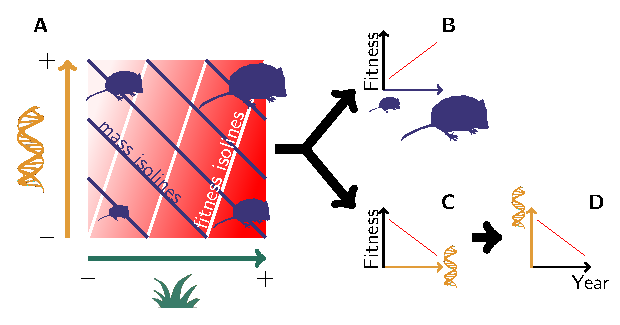
\includegraphics[width=0.9\textwidth]{FiguresStasis/Fig3}
\caption{\footnotesize \textbf{Schematic representation of why adaptive evolution goes opposite to apparent selection.} 
(\textbf{A}) Both genetic variation (orange) and environmental variation (green) contribute to phenotypic variation in mass (purple) in an additive and equivalent way: large voles are the result of genes for being large and of a favourable environment. Therefore, mass isolines form an angle of $45^\circ$ with both axes. However, the effect the fitness effect of the environmental component of mass variation is not the same as the fitness effect of the genetic component of mass variation: Fitness increases (the redder the fitter) with increasing environmental effects on mass, but decreases with increasing genetic effects on mass, as illustrated by fitness isolines (white). This pattern leads to (\textbf{B}) a phenotypic selection for heavier voles, along with (\textbf{C}) a ``genetic selection'' for lighter genotypes, thus leading to (\textbf{D}) an evolution towards lighter voles. Panel (\textbf{A}) should not be mistaken for a genotype-by-environment interaction: genetic and environmental effects are additive both for mass and for fitness. The additive effects on mass do not map on the additive effects on fitness, however.}
\label{fig:HypA}
\end{figure}

Indirect selection may be acting on body mass through one or more traits with negative genetic correlations with mass \parencite{Lande1983,Morrissey2012constraints}. However, the genetic correlations among the three morphological traits for which we have data\textemdash body mass ($m$), body length ($b$) and tail length ($t$)\textemdash are all positive (estimates and 95\%CI: $\rho_{m,b}=0.79$ $[0.06;0.93]$; $\rho_{m,t}=0.40$ $[0.01;0.66]$; $\rho_{t,b}=0.56$ $[-0.04;0.85]$), and the predicted response based on the multivariate breeder's equation (Fig. \ref{fig:gch}A MBE) is very similar to that based on its univariate counterpart (Fig. \ref{fig:gch}A UBE), as well as to that based on a multivariate breeder's equation constraining the correlations to zero (Fig. \ref{fig:gch}A MBE$_{\rho=0}$). Furthermore, for parent-offspring conflict between size and fertility to constrain the evolution of size, the genetic correlation between juvenile size and adult annual reproductive success should be negative \parencite{Rollinson2015b}. In our study population this correlation was 0.21, 95\%CI $[-0.24;0.74]$), arguing against a role for a trade-off between fertility and offspring size in driving the observed evolution toward smaller sizes. Although we cannot exclude that selection on other, unmeasured, traits does indirectly shape body mass evolution,  genetically correlated traits are not more likely to constrain than to facilitate adaptation \parencite{Agrawal2009}. This suggests that the counter-intuitive direction of evolution is really due to selective pressures acting on mass, but given that selection acts on phenotypes rather than genotypes, which aspect of an individual's body mass is the subject of negative selection? 

To identify the fitness component that is negatively associated with genes for being heavy, we computed sex- and age-specific genetic covariances between mass and fitness components. Whereas the genetic covariances between mass and both relative annual reproductive success and adult survival are close to zero in both sexes (Fig. \ref{fig:gch}B), the genetic covariance between mass and over-winter survival is negative in juveniles (-0.98 [-2.44;-0.18] on a logit scale, $p_\mathrm{MCMC}$=0.01). Because the genetic correlation between juvenile and adult mass is positive ($r_A=0.88$; 95\%CI [0.39;1]) and significantly different from 0 (p=0.004) but not 1 (p=0.35), selection on juvenile mass can shape genetic variance for mass at all ages, and thereby contribute to the observed negative genetic change \parencite{Chevin2015a}. While this shows that negative viability selection of juvenile mass is responsible for the genetic change toward smaller individuals, how come survival is higher for heavier phenotypes \emph{and} lighter genotypes? 

Juvenile mass covaries positively with both within- and between-year survival ($p=0.009$ and $p=1.3\times10^{-6}$, respectively). However, juveniles can only be captured when they first leave their burrow, at an age of approximately three weeks \parencite{Janeau1997} and a weight of 12 to 20 g, and they may continue to be captured until the end of the season, when they can reach weights of up to 50 g. Because of growth, mass measurements are therefore not directly comparable among juveniles. Indeed, at least part of the positive estimated selection on juvenile mass is likely to be mediated by the simultaneous increase, with age, of mass and of the probability of survival to the next year \parencite{Hadfield2008}. In addition, viability selection introduces non-random missing data, which results in biased estimates of viability selection on mass \parencite{Hadfield2008,Steinsland2014}. This led us to hypothesise that the positive phenotypic association between juvenile body mass and survival was largely the result of ontogeny non-random missing data, whereas the negative genetic association is driven by selection imposed by the necessity to have completed growth before the end of the growing season. 


The (co)variance decompositions presented above have the advantage that they do not make causative statements. For example, a genetic covariance describing the rate of evolution has a self-contained, tautological, meaning and does not make any assumptions with respect to its causes \parencite{Frank2012IV}. However, if we are to identify the target of juvenile viability selection, we must adopt a more traditional hypothesis testing framework. Although, as we emphasised above, inferring a causal relationship between a trait and fitness based on their covariance requires great care, we set out to test the hypothesis that when the period favourable for growth is limited, selection favours lighter juveniles, as they require less time to reach their adult size. 

To obtain an estimate of viability selection that is unbiased by growth and non-random missing data due to mass-dependent mortality occurring after the first capture \parencite{Hadfield2008}, we used a Bayesian model to simultaneously infer birth dates and growth curves for all juveniles observed at least once, irrespective of when and how often they have been captured. Although we cannot account for viability selection acting before the first capture, this model enabled us to quantify viability selection on age-corrected juvenile mass\textemdash i.e. asymptotic or predicted adult mass\textemdash, and thereby compare all individuals at the same developmental stage, irrespective of their fate. 

Inferred birth dates revealed that snow fallen during the preceding winter is a major ecological factor constraining the onset of reproduction in spring, with reproduction starting on average 40 days after the snow has melted (SE 4.5, $p=4\times 10^{-5}$) (Fig. \ref{fig:ResA}A). As a consequence, juveniles only have a limited amount of time to grow and reach their adult mass before the return of winter. As growth rate and predicted adult mass are slightly negatively correlated (correlation -0.077; 95\%CI [-0.150; -0.002]), juveniles with a smaller adult mass on average require less time to complete development. If individuals that have not completed development before the arrival of winter pay a survival cost, for example due to trade-offs between growth and vital physiological processes \parencite{Stearns1986,Owens1999}, this generates selection for small size, especially for juveniles born toward the end of the season (Fig. \ref{fig:ResA}D and Fig. \ref{fig:scheme}). 

To test this, we quantified the strength of survival selection acting on predicted adult mass, which was slightly negative when averaged over all years and the complete reproductive season ($p_\mathrm{MCMC}$=0.13), but interacted strongly and significantly with the number of days between birth and the first snowfall of that year ($p_\mathrm{MCMC}$=0.008). This implies that individuals born closer to the first snowfall are more strongly selected for a low adult mass, and that the length of the snow-free period in a given year determines the total selection experienced by the population in that year. Interestingly, at our field site, the length of the snow-free period in the years 2008 to 2014 has been significantly shorter than during the preceding six years (Fig. \ref{fig:ResA}B). The latter coincides with a period of exceptionally high snowfall, low temperatures and a long duration of snow cover, across the Swiss Alps \parencite{Beniston2012}.

Our model estimates that in 2006 and 2007, when the snow-free period was long (Fig. \ref{fig:ResA}B), most juveniles reached their adult mass before the first snowfall, and there was hence no selection on asymptotic mass ($\beta=-0.002$, SE= 0.0006, $p_\mathrm{MCMC}$=0.47, Fig. \ref{fig:ResA}C; D; \ref{fig:driftcomp}). However, in all subsequent years, the snow-free period was much shorter, and there was selection for a lower asymptotic mass ($\beta=-0.10$, SE=0.0008, $p_\mathrm{MCMC}$=0.009). This suggests that the shortening of the snow-free season, and thereby selection for lower asymptotic mass, is a novel phenomenon that the population is currently in the process of adapting to. Although model complexity and data availability prohibit disentangling genetic and environmental sources of variation in asymptotic mass among individuals and over time, and we cannot rule out the possibility that the selective pressure we identified is not causative \parencite{Morrissey2014}, the cohort born in 2013 had an estimated adult mass that was 1.02 g smaller than the cohort born in 2006 (p=0.05). This shrinkage is predicted to have increased population-level juvenile survival by 2.5\%, and to have contributed positively to population recovery (Fig. \ref{fig:pop}). 

\begin{figure}[h]
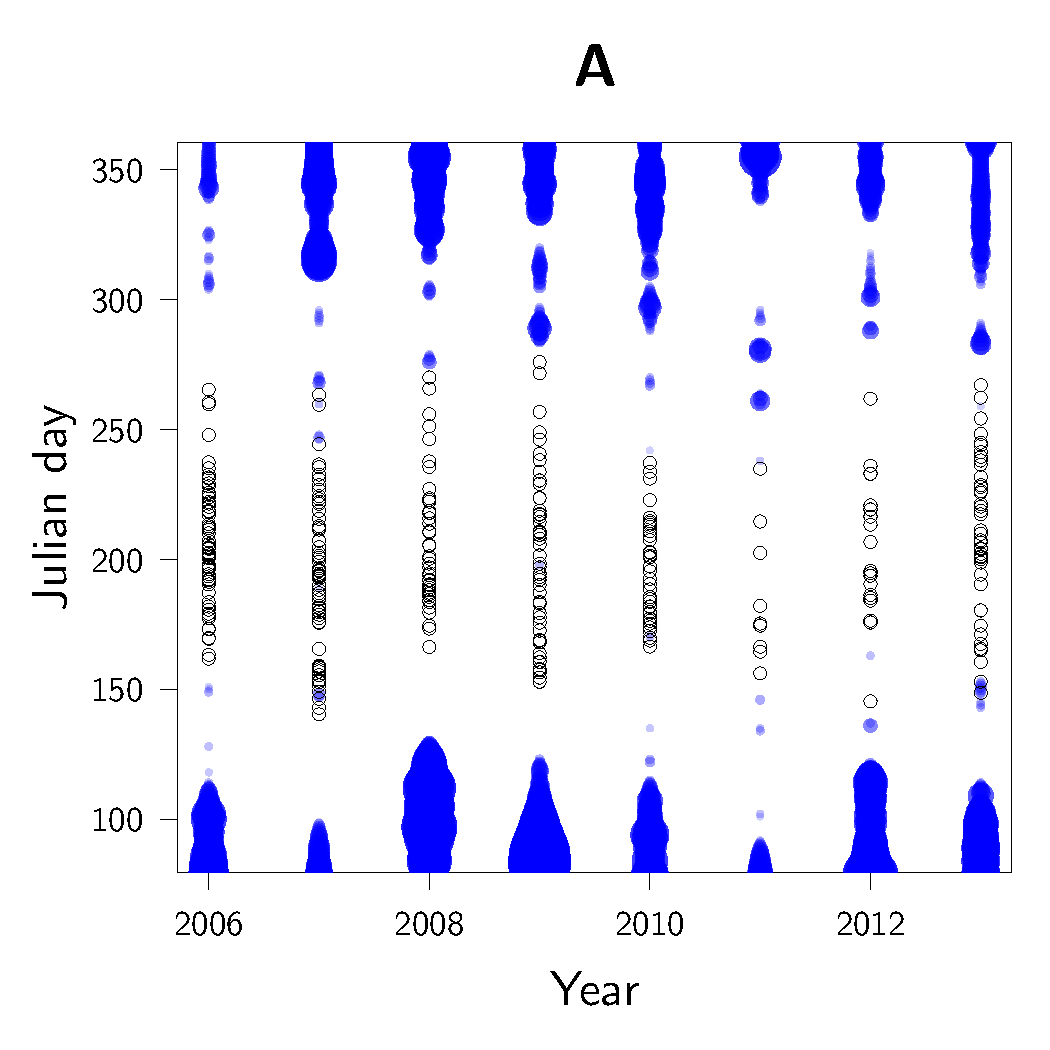
\includegraphics[width=0.5\textwidth]{FiguresStasis/BDsnow-1}
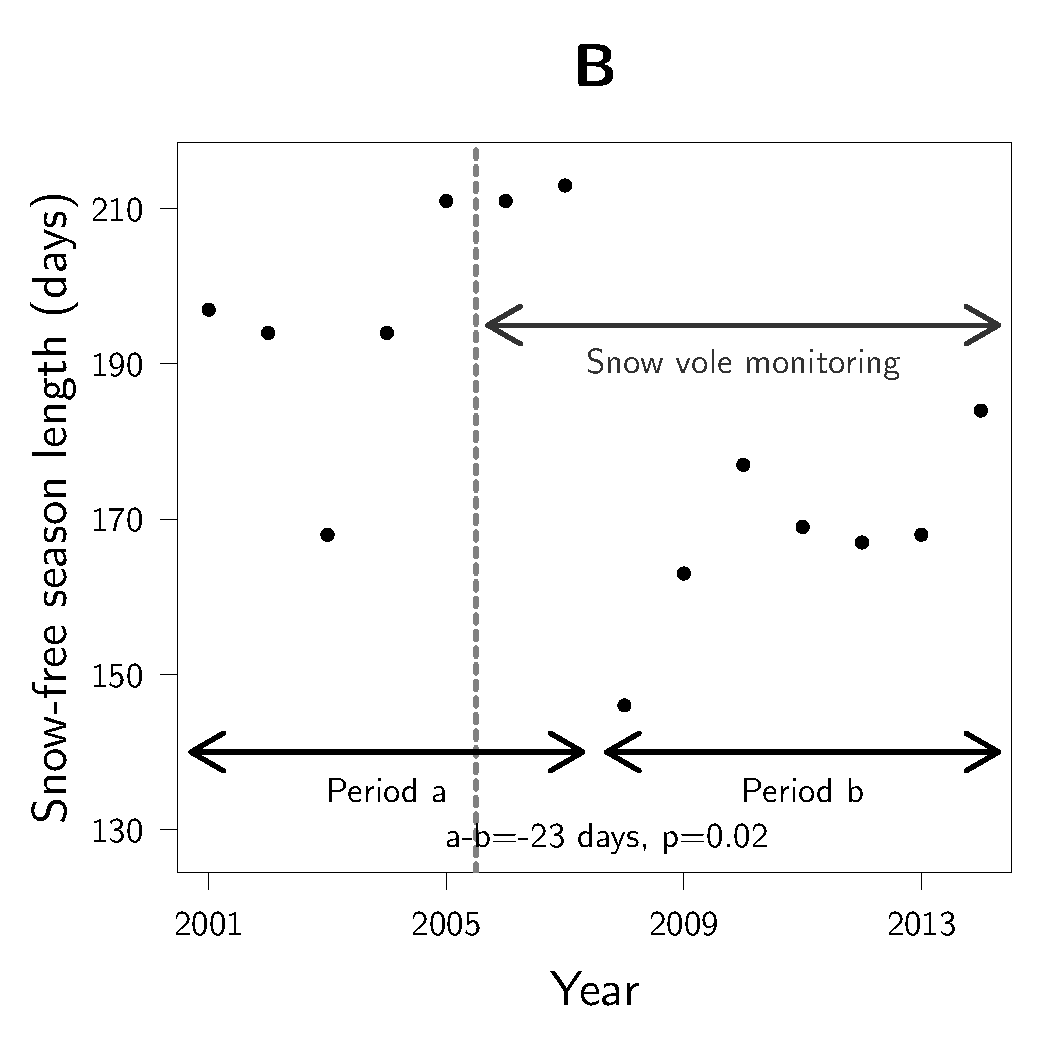
\includegraphics[width=0.5\textwidth]{FiguresStasis/Climatic_trend-1}
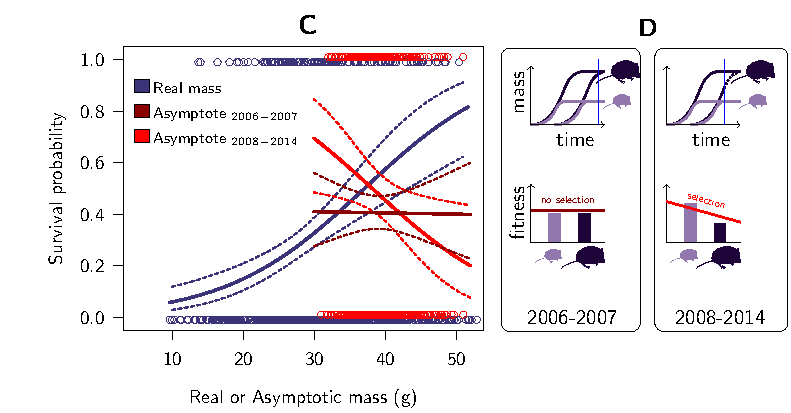
\includegraphics[width=1\textwidth]{FiguresStasis/Fig3b}
\caption{\footnotesize \textbf{Snow-free season, timing of reproduction and selection for asymptotic mass.} (\textbf{A}): Births (black dots) only occur during the snow free season (snow depth in blue), (\textbf{B}): which in 2008-2014 has been shorter than in the preceding 8 year. Therefore, (\textbf{C}) despite a positive phenotypic selection on body mass (blue), asymptotic mass was selectively neutral in 2006-2007 (brown), and was negatively selected in 2008-2014 (red), as a result of (\textbf{D}) the selective disappearance of heavy individuals that were born too close to the onset of winter (blue vertical line) during 2008-2014.}
\label{fig:ResA}
\end{figure}

\section{Conclusion}
We have exploited a case of apparent evolutionary stasis to gain a deeper insight into the evolutionary dynamics of natural populations, and the selective pressures that shape them. Whereas estimates of selection and evolution based on phenotypic data alone can easily mislead our understanding of the selective and evolutionary processes in natural populations, a quantitative genetic framework applied to individual-based long-term data allows us to unravel evolutionary and environmental changes over time, and to obtain unbiased estimates of selection. This has resolved a case of apparent evolutionary stasis, and provided a comprehensive empirical demonstration of contemporary adaptive evolution in response to a climatic fluctuation. 

\section{Methods}
\paragraph{Snow vole monitoring.}
Monitoring of the snow vole population began in 2006 and the present work uses data collected until the fall of 2014. The snow vole monitoring was authorised by the \textit{Amt f\"{u}r Lebensmittelsicherheit und Tiergesundheit}, Chur, Switzerland. The study site is located at around 2030m above sea level, in the central eastern Alps near Churwalden, Switzerland ($46^{\circ}$48' N, $9^{\circ}$34' E). It consists of scree, interspersed with patches of alpine meadows and surrounded by habitat unsuitable for snow voles: a spruce forest to the West, a cliff to the East and large meadows to the North and South. In accordance with it being considered a rock-dwelling specialist \parencite{Janeau1997}, at our study site it is almost never captured outside of the rocky area. Given that it is ecologically fairly isolated, we are able to monitor the whole population.
Trapping throughout the whole study area takes place during the snow-free period, between late May and mid-October. One trapping session consists of four trapping nights. Analyses presented here are based on a total of two (in one year), three (in three years) or five (in five years) trapping sessions per season.
All newly-captured individuals weighing more than 14 g are marked with a subcutaneous passive transponder (PIT, ISO transponder, Tierchip Dasmann, Tecklenburg). Additionally, an ear tissue sample is taken (maximum 2 mm in diameter) using a thumb type punch (Harvard Apparatus) and stored in 100\% ethanol at $-20^{\circ}\mathrm{C}$. DNA extracted from these samples is genotyped for 18 autosomal microsatellites developed for this population \parencite{Wandeler2008}, as well as for the \textit{Sry} locus to confirm the sex of all individuals. Finally, another Y-linked marker as well as a mitochondrial marker is used check for errors in the inferred pedigree (see below). An identity analysis in \verb+CERVUS+ v.3.0 \parencite{Marshall1998} allows us to identify animals sampled multiply, either because they lost their PIT, or because at their first capture as a juvenile they were too small to receive a PIT.
All the analyses were carried out in \verb+R+ \parencite{R2014}. Specific packages are referenced below.

\paragraph{Pedigree inference.}
Parentage was inferred by simultaneously reconstructing paternity, maternity and sibship using a maximum likelihood model in \verb+MasterBayes+ \parencite{Hadfield2006}. Parentage was assigned using a parental pool of all adults present in the examined year and the previous year, assuming polygamy and a uniform genotyping error rate of 0.5\% for all 18 loci. As it is known that in rare cases females reach sexual maturity in their year of birth \parencite{Janeau1997}, we matched the genotypes of all individuals against the genotypes that can be produced by all possible pairs of males and females. We retrieved the combinations having two or less mismatches (out of 18 loci) and ensured that parental links were not circular and were temporally consistent. This way, we identified eight young females as mothers of animals born in the same year, with a known father but a mother not yet identified. All of these females were relatively heavy ($>$33 g) at the end of the season and their home-ranges matched those of their putative offspring.
Finally, the pedigree was checked using a polymorphic Y-linked locus developed for this population \parencite{Wandeler2011}, as well as a fragment of the mitochondrial DNA control region, amplified using vole specific primers \parencite{Haring2000}. There were no inconsistencies between the transmission of these three markers and the reconstructed pedigree.
The final pedigree had a maximum depth of 11 generations and a mean of 3.8 generations. It consisted of 987 individuals with 458 full-sibling pairs, 3010 half-sibling pairs, 764 known maternities and 776 known paternities, so that, excluding the base population, 86\% of the total parental links were recovered.

\paragraph{Traits.}
The recapture probability from one trapping session to the next was estimated to be 0.924 (SE 0.012) for adults and 0.814 (SE 0.030) for juveniles using mark-recapture models. Thus, with three trapping session a year, the probability not to trap an individual present in a given year is below $10^{-3}$. Not surprisingly, no animal was captured in year $y$, not captured in $y+1$, but captured or found to be a parent of a juvenile in $y+2$ or later. Therefore, capture data almost perfectly matches over-winter survival. However, as is almost always the case in these type of studies, we are unable to separate death from permanent emigration. Importantly however, as both have the same consequences on the population level, this does not affect our evolutionary predictions.

Annual and lifetime reproductive success (ARS and LRS, respectively) were defined as the number of offspring attributed to an individual in the pedigree, either over a specific year or over its lifetime. 56 individuals born of local parents were not captured in their first year, but only as adult during the next summer, probably because they were born late in the season and we had only few opportunities to catch them. This means that we miss a fraction of the juveniles that are not observed in their first year and die, or emigrate, during the following winter. We acknowledge that this means that our measures of ARS and LRS partly conflate adult reproductive success and the viability of those juveniles that were never observed, but our measures are the most complete measures of reproductive success available in this system.

We used relative LRS ($\omega$) as proxy for fitness \parencite{Lande1983}, where $ \omega_{i} = \frac{\mathrm{LRS}_{i}}{\frac{1}{N_{s,t}}\sum_{j=1}^{N_{s,t}} {\mathrm{LRS}_{j,t}}} $. Here, $N_{s,t}$ is the number of individuals of same sex as the focal individual $i$, present in the cohort $t$, so that $\frac{1}{N_{s,t}}\sum_{j=1}^{N_{s,t}} {\mathrm{LRS}_{j,t}}$ is the sex-specific, cohort-specific mean of LRS. The latter is required as the mean LRS differs between males and females due to imperfect sampling \parencite{Morrissey2012sts}. In addition, we used cohort-specific means in order to account for variations in population size.

Generation time was defined as the mean age of parents at birth of their offspring\parencite{Charleworth1994}.

Mass ($m$) was measured to the nearest gram with a spring scale. Both body length ($b$), measured from the tip of the nose to the base of the tail, and tail length, measured from the tip to the base of the tail ($c$), were measured to the closest mm with a calliper while holding the animal by the tail. 

\paragraph{Selection.}
Selection differentials were estimated using bivariate linear mixed models, as the individual-level covariance between fitness and mass (corrected for sex, age and cohort). However, while this provides the best estimate of the within-generation change in trait mean due to selection \parencite{Lande1983}, because the distribution of fitness is not Gaussian, it cannot be used to estimate confidence intervals. Hence, the statistical significance of selection was tested using a univariate over-dispersed Poisson generalized linear mixed model (GLMM) in which LRS was modelled as a function of individual standardized mass and including sex and age as covariates and cohort as a random effect. Note that the latter estimates the effect of mass on a transformed scale, and therefore cannot be directly used to quantify an effect of selection on the original scale measured in grams \parencite{Mitchell-Olds1987}. The significance based on the basis of the GLMM was confirmed by non-parametric bootstrapping. Similarly, we tested for the significance of selection through ARS only, using an over-dispersed Poisson GLMM including sex as a fixed effect, and year and individual as random effects. 

The estimation of survival selection is facilitated by the fact that the year-to-year individual recapture probability is effectively 1. Therefore, selection on year-to-year survival was tested for by a binomial GLMM. This model included sex, age and their interaction as fixed effects, and year as a random effect.

In order to integrate the uncertainty in the estimation of selection with the uncertainty in the estimation of heritability when predicting the rate of evolution, selection differentials and gradients were also obtained from the multivariate animal model presented below.

\paragraph{Quantitative genetic analyses.}
We used uni- and multivariate animal models to estimate additive genetic variances, covariances and breeding values \parencite{henderson1984,Lynch1998,Kruuk2004} with \verb+MCMCglmm+ \parencite{Hadfield2010a}. All estimations were carried out in a Bayesian framework in order to propagate uncertainty when computing composite statistics such as heritabilities and rates of genetic change \parencite{Stinchcombe2014}. All estimates provided in the text are posterior modes and credibility intervals are highest probability density intervals at the 95\% level.
All the animal models were run for 1,300,000 iterations with a burnin of 300,000 and a thinning of 1,000, so that the autocorrelations of each parameter chain was less than $0.1$. Convergence was checked graphically and by running each model twice.

\paragraph{Univariate models: }
We first carried out univariate model selection, fitting models without an additive genetic effect, to determine which fixed and random effects to include. Based on AICc \parencite{Burnham2002c}, and fitting the models by Maximum of Likelihood in \verb+lme4+ \parencite{Bates2014a}, we obtained a model that predicts the mass $m_{i,t}$ of individual $i$ at time $t$ by: age, as a factor (juvenile or adult); sex as a factor; the interaction between age and sex; Julian dates and squared Julian dates, which were centered and divided by their standard deviations in order to facilitate convergence; the interaction between age and Julian date; the interaction between sex and Julian date; the three way interaction between age, sex and Julian dates; a random intercept for individual; and a random intercept for year. The inclusion of year accounts for non-independence of observation within years, while individual accounted for the non-independence of repeated measurements made on the same individual \parencite{Kruuk2007}. 
We then fitted an animal model by adding a random intercept modelling variance associated with mother identity \parencite{Kruuk2004}, and a random intercept modelling additive genetic variance. Although it was not included in the best models, we kept inbreeding coefficient (estimated from the pedigree) as a covariate, because leaving it out could bias the later estimation of additive genetic variation \parencite{deBoer1993}. Nevertheless, animal models fitted without this covariate gave indistinguishable estimates.

\paragraph{Multivariate models: }
Univariate animal models can be expanded to multivariate models in order to estimate genetic correlations, genetic gradients and genetic differentials.

\begin{align*}
[\boldsymbol{m},
\boldsymbol{l},
\boldsymbol{t},
\boldsymbol{\omega}]
\sim
\boldsymbol{bX}+\boldsymbol{D_1a}+\boldsymbol{D_2m}+\boldsymbol{D_3p}+\boldsymbol{D_4y}+\boldsymbol{Ir.}\\
\end{align*}
Here $\boldsymbol{X}$, $\boldsymbol{D_1}$, $\boldsymbol{D_2}$, $\boldsymbol{D_3}$ and $\boldsymbol{D_4}$ are design matrices relating observations to the parameters to estimate, $\boldsymbol{b}$ is a matrix of fixed effects, $\boldsymbol{a}$, $\boldsymbol{m}$, $\boldsymbol{p}$ and $\boldsymbol{y}$ are random effects accounting for the variance associated with breeding value, mother, permanent environment and year, respectively. The fixed part of the model matches that used for each trait in univariate models.

The most important aspect of this model is that $\boldsymbol{a}$, the matrix of breeding values, follows a multivariate normal distribution:
\begin{equation}\boldsymbol{a}
\sim MVN\left(\boldsymbol{0},
\boldsymbol{A \otimes G}
\right)
\end{equation}
where $\boldsymbol{A}$ is the relatedness matrix describing the relatedness among all individuals, and $\boldsymbol{G}$ is the G-matrix, containing the additive genetic variances and covariances among all traits.\\

\begin{equation}
\boldsymbol{G}=\begin{pmatrix}
\sigma_{A}^2(m) & \sigma_{A}(m,l) & \sigma_{A}(m,t) & \sigma_{A}(m,\omega)\\
\sigma_{A}(m,l) & \sigma_{A}^2(l) & \sigma_{A}(l,t) & \sigma_{A}(l,\omega)\\
\sigma_{A}(m,t) & \sigma_{A}(l,t) & \sigma_{A}^2(t) & \sigma_{A}(t,\omega)\\
\sigma_{A}(m,\omega) & \sigma_{A}(l,\omega) & \sigma_{A}(t,\omega) & \sigma_{A}^2(\omega)\\
\end{pmatrix}.
\end{equation}

For any trait $z$, $\sigma_{A}(z,\omega)$ is the genetic differential, that is, the predicted rate of evolutionary change according to Robertson's secondary theorem of natural selection, or Price equation applied to genetic variation \parencite{Robertson1966, Price1970, Morrissey2012sts}. The Price equation is generally presented as a prediction of evolutionary change over the next generation, but it has also been used as a description of change \parencite{Heywood2005, Frank2012IV, Coulson2008}. We use this prediction retrospectively, as an estimation of the mean evolutionary change that has occurred during the study period, which makes the assumption that $\omega$ is a good measure of fitness, because when ``real fitness'' is used, the equation is a mathematical tautology, i.e. it is exact \parencite{Frank2012IV}. A deviation from this perfect fitness measure could come from random Mendelian segregation or systematic meiosis distortion. Our results were robust to the use of an annualized measure of fitness (annual reproductive success plus twice survival), and to standardizing fitness across all individuals, within years, within cohorts, and within sexes.

For two traits $z$ and $y$, the genetic correlation is $\frac{\sigma_{A}(z,y)}{\sigma_{A}(z)\sigma_{A}(y)}$.
The vector of selection differentials on the three traits ($\boldsymbol{S}$) was estimated as the sum of the vectors of covariances between traits and $\omega$ in the variance-covariance matrices for $\boldsymbol{a}$, $\boldsymbol{p}$ and $\boldsymbol{r}$; which was equivalent to the selection differential computed in the paragraph on selection above. We excluded the among-year level covariance from the selection differential, because (i) covariation between mass and fitness at the level of year does not correspond to selection as it does not occur among individuals (ii) due to the standardization of relative fitness at the level of cohorts, the among year variance and covariances involving $\omega$ were effectively zero ($\sigma_{Y}^2(\omega)<10^{-8}$). 
Let $\boldsymbol{G^\prime}$ be a subset of $\boldsymbol{G}$ excluding the column and the row that contain $\omega$.
The vector of selection gradients on the three traits ($\boldsymbol{\beta}$) was estimated as $\boldsymbol{(G^\prime+P^\prime+R^\prime)^{-1}S}$, where $\boldsymbol{P^\prime}$ and $\boldsymbol{R^\prime}$ are the equivalent of $\boldsymbol{G^\prime}$ for permanent environment effects and for residuals, respectively.

The prediction of the multivariate breeders equation is obtained by $\Delta \overline{\boldsymbol{Z'}}=\boldsymbol{G^\prime \beta}$, while the multivariate breeders equation ignoring genetic correlations is obtained by multiplying the $\boldsymbol{G^\prime}$ matrix by the identity matrix\parencite{Morrissey2012constraints}: $\Delta \overline{\boldsymbol{Z'}}=\boldsymbol{(G^\prime \times I)\beta}$.

To investigate the potential role of parent-offspring conflict, we estimated the genetic correlation between parental ARS and offspring mass using a bivariate animal model. For juvenile mass, we used predicted adult mass (i.e. age-corrected juvenile mass; see below). The model included sex, Julian dates and squared Julian dates as fixed effects for offspring mass, and only sex for ARS. 
\begin{align*}
[\boldsymbol{m_O},
\boldsymbol{ARS_P}]
\sim
\boldsymbol{bX}+\boldsymbol{D_1a}+\boldsymbol{D_2y}+\boldsymbol{Ir.}\\
\end{align*}

\paragraph{Test of genetic correlations: }
We used \verb+ASReml-R+ \parencite{Gilmour2014, Butler2009} to test the genetic correlation between mass in adults and in juveniles against 1 and 0, by considering them as two separate traits. We first ran an unconstrained model and then reran it with the genetic correlation parameter set to 0.99 (and not exactly to 1 because \verb+ASReml+ cannot invert matrices with perfect correlations), or 0 respectively. The fit of the unconstrained model was then compared to that of the two constrained models using a likelihood ratio test with one degree of freedom \parencite{Wilson2009}.

\paragraph{Birth date and growth prediction: }
Using the Bayesian programming environment \verb+JAGS+ \parencite{Plummer2003}, we fitted a multivariate Bayesian model to mass measurements of all 613 juveniles with mass data, and to their overwinter survival. The model simultaneously estimated individual growth curves\textemdash that is onset of growth (although this is referred to as ``birth date'' hereafter, this actually is the projected time when mass was zero, i.e. at conception), individual growth rates and asymptotic masses of all juveniles\textemdash and the effect of asymptotic mass on overwinter survival. The model clustered juveniles from the same mother born in the same year into litters (see e.g. \parencite{Cornulier2009} for a similar approach), assuming a maximum of five litters per year and assuming that successive litters are at least 20 days apart \parencite{Janeau1997}. Preliminary model selection, assuming no differences in asymptotic masses among individuals, selected a monomolecular growth model ($\Delta \mathrm{DIC} > 80$) over Gompertz and logistic models, as defined in \parencite{English2012}. The model accounted for measurement error in mass, assuming that the standard deviation of the errors was that observed in animals measured multiple times on the same day (2.05g).
In order to estimate the overall viability selection on asymptotic mass, we performed within the model a logistic regression of year-to-year survival on sex and asymptotic mass. In order to test for the effect of the length of snow free period on the selection on asymptotic mass, we reran the full model including time until the first snow fall and its interaction with asymptotic mass in the logistic regression. We use the estimates of these two models to predict the survival probability as a function of asymptotic mass for every year, or for groups of years, depending on the distribution of birth dates and on the timing of the first snow fall. 


Three MCMC chains were run for 6,300,000 iterations, with a burnin of 300,000 and a thinning of 6,000. Convergence was assessed by visual examination of the traces, and by checking that the $\hat{R}<1.01$. Convergence was not achieved for the litter affiliations of 25 individuals as well as for one asymptotic mass, thus generating a bit more uncertainty in the estimations. The fit of the model was assessed using posterior predictive checks on the predictions of individual masses (p=0.46) and survival probabilities (p=0.49).  
The \verb+JAGS+ code for this model can be found at \url{https://github.com/timotheenivalis/SelRepSel}.

\section*{Acknowledgements}
Thanks to Lauren Richardson, Tim Coulson, Alastair Wilson and two anonymous reviewers for constructive comments. Thanks to Wolf U. Blanckenhorn, Jarrod D. Hadfield, Lukas F. Keller, Marc K\'{e}ry, Hanna Kokko, Chelsea J. Little, Pirmin Nietlisbach, Barbara Tschirren and Ashley E. Latimer for comments and discussions on earlier versions of this work. Thanks also to the many field helpers. Weather data were provided by MeteoSwiss. The snow vole monitoring was authorised by the \textit{Amt f\"{u}r Lebensmittelsicherheit und Tiergesundheit}, Chur. Switzerland. T.B. is funded by a Swiss National Science Foundation project grant (\verb|31003A_141110|) awarded to EP. 

\printbibliography[heading=subbibliography]

\clearpage
\section{Supplementary information}

\begin{figure}[ht]
\centering
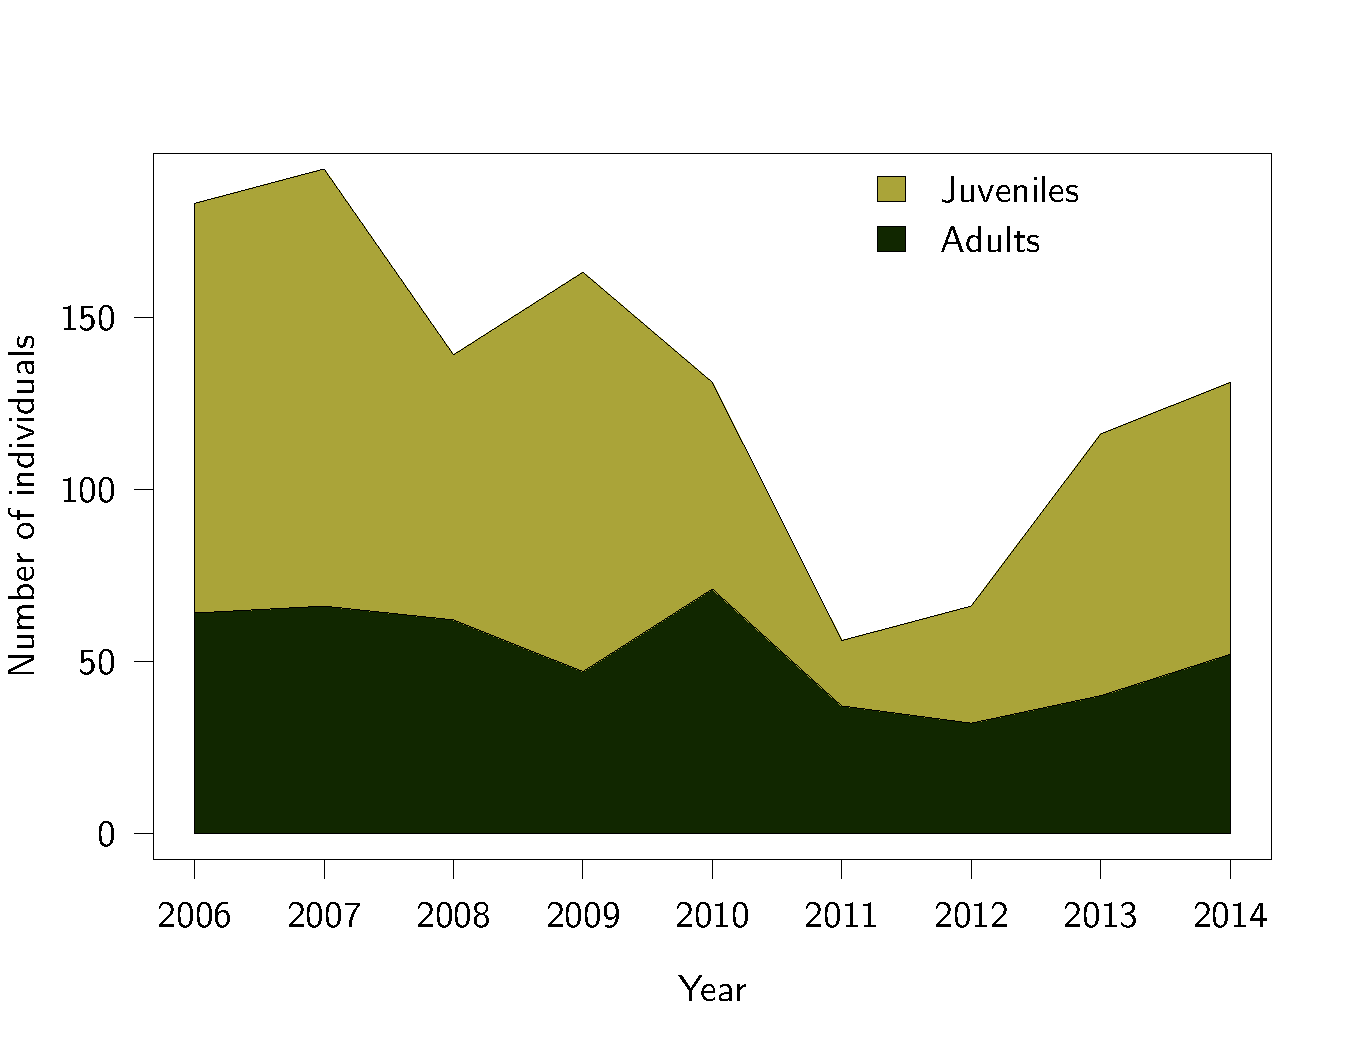
\includegraphics[width=0.5\textwidth]{FiguresStasis/PopulationTrend-1}
\caption{\footnotesize \textbf{Temporal variation in population size and age-structure.} Number of individual adults and of juveniles captured in each year.}
\label{fig:pop}
\end{figure}

\begin{figure}[h]
\centering
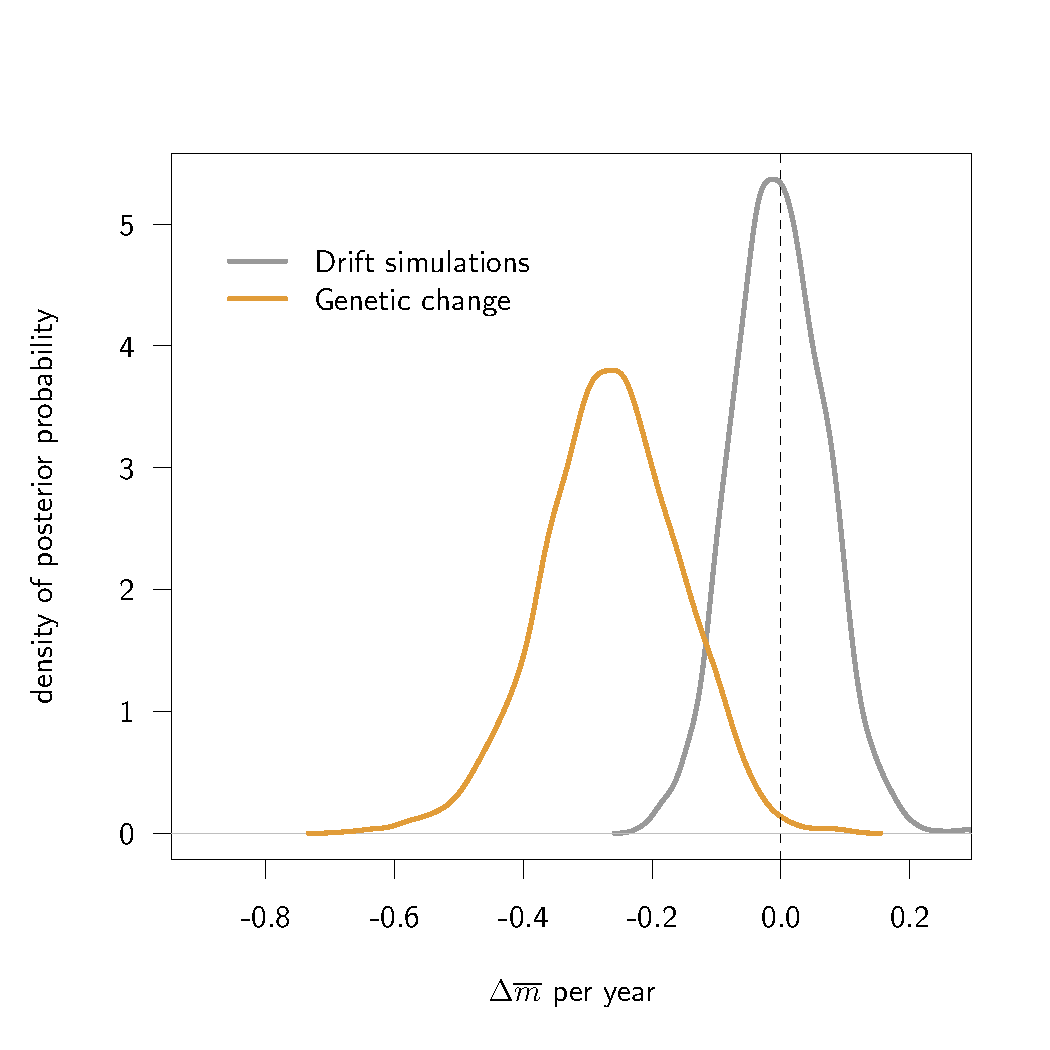
\includegraphics[width=0.5\textwidth]{FiguresStasis/Drift-1}
\caption{\footnotesize \textbf{Estimation of the rate of genetic change and rate of change expected under drift.} The posterior distributions of the realized rate of genetic change, estimated by the Price equation, exceeds that expected under genetic drift $p=0.009$.}
\label{fig:drift}
\end{figure}

\begin{figure}[ht]
\centering
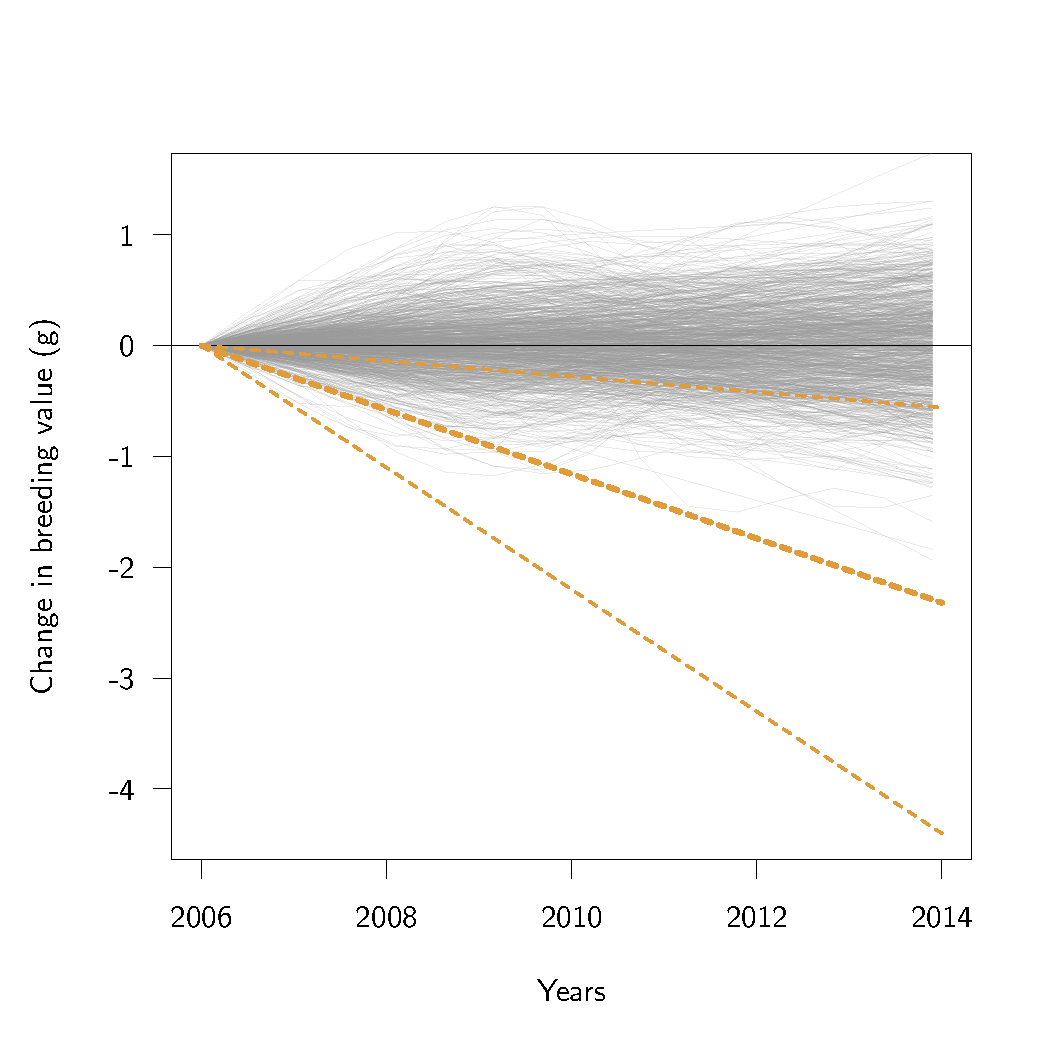
\includegraphics[width=0.5\textwidth]{FiguresStasis/DriftComp-1}
\caption{\footnotesize \textbf{Estimation of the time-trajectory of genetic change and evolutionary trajectories simulated with drift only.} Evolution of breeding values for mass are shown relative to the year 2006. The yellow lines show the mode and 95\% credibility interval of the rate of evolution estimated by the Price equation within an animal model. The gray lines show 1,000 simulations of genetic drift, based on the real population pedigree and on the posterior distribution of genetic variance for mass estimated by the animal model. The probability that the observed rate of evolution happened due to drift is only 0.009, less than could be understood from the overlap between the two distribution. It is, however important to notice that the two distributions are not independent, but that small (/large) values of change due to drift are simulated for small (/large, respectively) posterior samples of estimate rate of evolution.}
\label{fig:driftcomp}
\end{figure} 


\begin{figure}[ht]
\centering
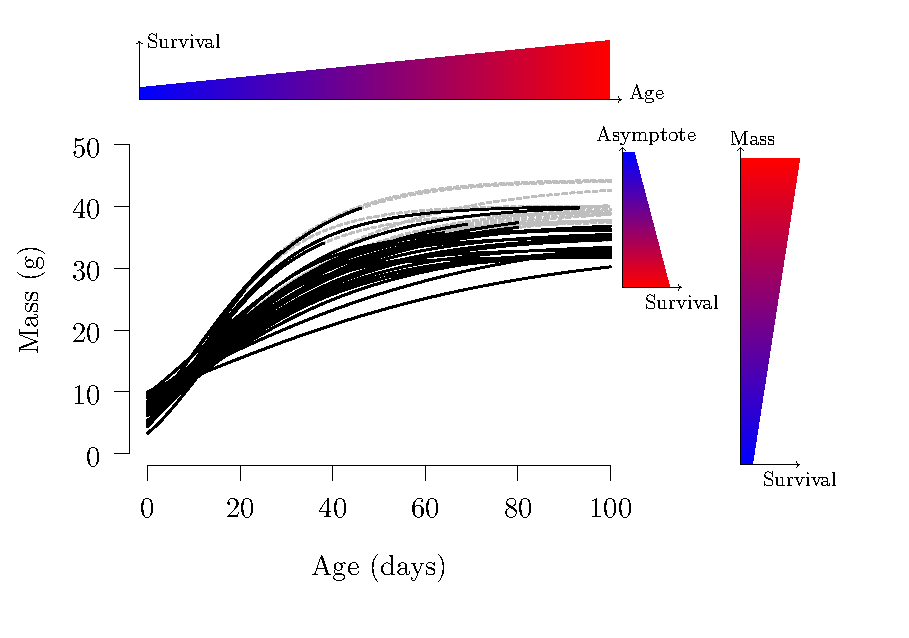
\includegraphics[width=\textwidth]{FiguresStasis/schemeSelectionAM}
\caption{\footnotesize \textbf{Conceptual illustration of the selection for asymptotic mass despite apparent selection for mass.} Black lines represent simulated individual growth trajectories, and they are prolonged by grey dashed lines after an individual death. The probability of surviving between the time of measurement and the next year increases with age. Because mass increases with age, there is apparent selection favouring heavier individuals. However, it is still possible for viability selection at a given developmental stage, such as asymptotic mass, to be negative. Because genetic variation is related to asymptotic mass, but not to age, the expected genetic change will be toward lower masses.}
\label{fig:scheme}
\end{figure}